\chapter{sounds}
\label{sec:listing}
\lstset{style=68KStyle}

The sound effects in Tempest 2000 are stpred in the game as Pulse Code Modulation (PCM) data. This is the most common format for storing
raw audio and flavors of it are used in everything from CDs to telephony. PCM data is as simple as a stream of numbers. Each of the numbers
is between a lower and upper limit:, for example between -128 and 128. If you plot enough of these numbers along a graph you get what looks like
a wave. This is pretty much the sound wave, the analog version of our digital values. If you put these values through the right piece of hardware,
such as a Digital Analog Converter (DAC) you can get a sound out the other side.

\begin{figure}[H]
    \centering
    \begin{adjustbox}{width=7cm,center}
      \frame{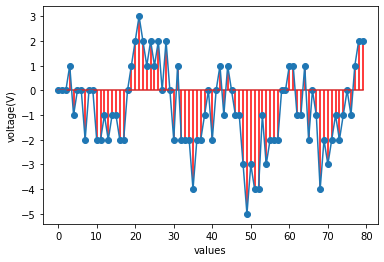
\includegraphics[width=4cm]{src/sounds/sample.png}}%
    \end{adjustbox}
  \caption{A sample of 80 bytes plotted as a wave graph.}
\end{figure}

The PCM data in Tempest 2000's sound samples is nothing more than this series of bytes, each one representing a value between -128 and 128, which can
be converted into sound. A single series of bytes will give us one 'channel' of sound, i.e. a mono sound sample. What we actually have are stereo
sound samples so each sample contains two channels. The simplest way of incorporating two separate channels in the sample (one for the left speaker
and one for the right) is to interleave them, in alternating bytes. We can see that this is the way the Tempest samples are encoded if we split out
an arbitrary sample into separate streams of alternate bytes and graph them.

\begin{figure}[H]
    \centering
    \begin{adjustbox}{width=12cm,center}
      \frame{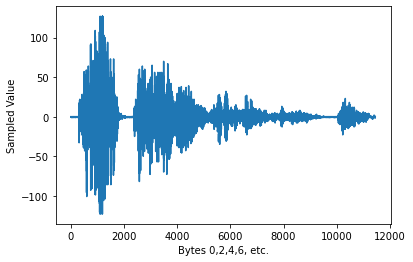
\includegraphics[width=4cm]{src/sounds/samplel.png}}%
      \hspace{0.5cm}
      \frame{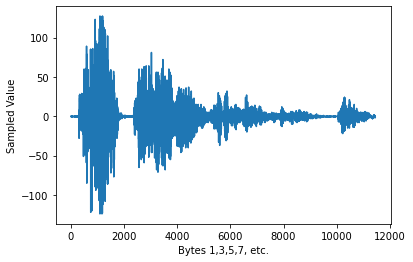
\includegraphics[width=4cm]{src/sounds/sampler.png}}%
    \end{adjustbox}
  \caption{Plotted sound waves for the left and right channels respectively.}
\end{figure}


\begin{lstlisting}
  samtab       EQU $9ac800
\end{lstlisting}

\begin{lstlisting}[caption=The contents of \icode{samtab} at \icode{\$9AC800}.]
;                             Prio-                                  Repeat     Repeat
;     Name                    rity   Period Start      Length        Start      Length      
;     ----------------------  -----  ------ ---------  -------  --   ---------  ------- ---
dc.b 'Engine Noise 1      ', $0001, $01ac, $009acd00, $0011a0, $00, $009acd02, $00119e, $00
dc.b 'Player Shot Normal 2', $0002, $01ac, $009adea4, $0008e8, $00, $009adea4, $000000, $00
dc.b 'Engine Noise        ', $0003, $01ac, $009ae290, $003378, $00, $009aee9e, $002594, $00
dc.b 'Player Death        ', $0004, $00d6, $00000000, $00549a, $00, $00000000, $000000, $00
dc.b 'Player Death 2      ', $0005, $01ac, $00000000, $002458, $00, $00000000, $000000, $00
dc.b 'Player Shot Normal  ', $0006, $01ac, $009b160c, $0007a4, $00, $009b160c, $000000, $00
dc.b 'Player Jump         ', $0007, $01ac, $009b1db4, $0018de, $00, $009b1db4, $000000, $00
dc.b 'Crackle             ', $0008, $00d6, $009b3696, $004594, $00, $009b3696, $000000, $00
dc.b 'Cleared Level       ', $0009, $01ac, $009b7c2e, $0037a2, $00, $009b7c2e, $000000, $00
dc.b 'Warp                ', $000a, $0238, $009bb3d4, $006ec8, $00, $009bb3d4, $000000, $00
dc.b 'Large Explosion     ', $000b, $01ac, $009c22a0, $0050c2, $00, $009c22a0, $000000, $00
dc.b 'Powered Up Shot     ', $000c, $01ac, $009c7366, $001976, $00, $009c7366, $000000, $00
dc.b 'Get Power Up        ', $000d, $01ac, $009c8ce0, $001aea, $00, $009c8ce0, $000000, $00
dc.b 'Tink For Spike      ', $000e, $00fe, $009ca7ce, $00040e, $00, $009ca7ce, $000000, $00
dc.b 'NME At Top Of Web   ', $000f, $01ac, $009cabe0, $00001e, $00, $009cabe0, $000000, $00
dc.b 'Pulse For Pulsar    ', $0010, $0358, $009cac02, $0019fe, $00, $009cac02, $000000, $00
dc.b 'Normal Explosion    ', $0011, $00d6, $009cc604, $002ab6, $00, $009cc604, $000000, $00
dc.b 'Extra Explosion     ', $0012, $0358, $009cf0be, $0018ca, $00, $009cf0be, $000000, $00
dc.b 'Static or Pulsar    ', $0013, $011c, $009d098c, $003fe4, $00, $009d098c, $000000, $00
dc.b 'Pulsar Pulse        ', $0014, $0358, $009d4974, $000f0c, $00, $009d4974, $000000, $00
dc.b 'Off Shielded NME    ', $0015, $00aa, $009d5884, $0027ca, $00, $009d5884, $000000, $00
dc.b 'Excellent           ', $0016, $0200, $009d8052, $005976, $00, $009d8052, $000000, $00
dc.b 'Superzapper Recharge', $0016, $0200, $009dd9cc, $00a958, $00, $009dd9cc, $000000, $00
dc.b 'yes                 ', $0018, $0200, $009e8328, $005a6c, $00, $009e832a, $005a6a, $00
dc.b 'oneup               ', $0019, $0200, $009edd98, $0043ae, $00, $009edd98, $000000, $00
dc.b 'screeeam            ', $001a, $0200, $009f214a, $004568, $00, $009f214a, $000000, $00
dc.b 'sexy yes 1          ', $001b, $0200, $009f66b6, $002c54, $00, $009f66b6, $000000, $00
dc.b 'sexy yes 2          ', $001c, $0200, $009f9362, $003236, $00, $009f9362, $000000, $00
dc.b 'tink                ', $001e, $0200, $009fc59c, $0005ce, $00, $009fc59c, $000000, $00
dc.b 'zero                ', $001f, $0200, $009fcb6e, $000008, $00, $009fcb6e, $000000, $00
dc.b 'dummy               ', $0020, $0200, $009fcb7a, $00a1d8, $00, $009fcb7a, $000000, $00
\end{lstlisting}


%\begin{figure}[H]
%{
%\setlength{\tabcolsep}{1.0pt}
%\setlength\cmidrulewidth{\heavyrulewidth} % Make cmidrule = 
%\begin{adjustbox}{width=14cm,center}
%\begin{tabular}{ccc}
%\toprule
%Spectrogram & Amplitude & Sound \\
%\midrule
%  \makecell[l]{
%    \includegraphics[width=6cm]{sound_effects/planetWarpSoundEffect.wav-spec.png}%
%  } &
%  \makecell[l]{
%    \includegraphics[width=6cm]{sound_effects/planetWarpSoundEffect.wav-amp.png}%
%  } &
%  \makecell[l]{
%    \textattachfile{src/sound_effects/sounds/planetWarpSoundEffect.wav}{
\includegraphics[width=1cm]{sound_effects/sounds/play.png}}
%  } \\
%  \addlinespace
%    \bottomrule
%    \end{tabular}
%  \end{adjustbox}
%}\caption{}
%\end{figure}
